\chapter{LDA Model Monitoring in Distributed Systems}
\label{chap:secondchap}

\section{Related Work}
Monitoring dynamic data streams is a broad topic that has been addressed in different research communities. Within this field, we focus on detecting a change in the data stream that renders the prediction model invalid. 
In distributed settings, this problem is even harder and referred to as \textit{distributed monitoring}, and it is concerned with designing local tests for monitoring a function that is defined globally over all the nodes in the system.
Our approach to this problem is to define a constraint over the local data (at each node) that guarantees the validity of the global model. If local data (in one or more nodes) does not meet the local condition, it leads to synchronization. The synchronization process has large communication costs, and the goal of the distributed monitoring methods is thus to minimize the number of synchronizations. Most of the work on distributed monitoring has been concerned with simple functions of the data, such as linear functions in the work of ~\cite{keralapura2006communication} and ~\cite{kashyap2008efficient} or monotonic functions in the work of \cite{michel2005klee}.
For non-linear functions, examples include work on monitoring the value
of a single-variable polynomial as in the work of ~\cite{shah2008handling},
and eigenvalue perturbation as in the work of ~\cite{huang2007communication}.
While the previous work handled specific families of functions, we chose to use \textit{geometric} approach for monitoring \textit{arbitrary} functions over distributed streams, as was proposed, later extended and generalized in \cite{sharfman2007geometric, keren2014geometric, keren2012shape}. A recently introduced work by ~\cite{gabel2015monitoring} on monitoring Least Square Regression (LSR) using geometric monitoring is the closest to ours, but our problem is more complex: unlike the global scatter matrix (required by LSR) the global covariance matrix (required in LDA) is not the mean of the local covariance matrices which makes the monitoring problem more much harder.

\section{Problem Definition}
We first describe the Linear Discriminant Analysis (LDA) algorithm and then define the monitoring problem. 

\subsection{Linear Discriminant Analysis}%\\ \par
LDA seeks a linear combination of features that characterize or separate two or more classes of samples.
The resulting combination may be used as a linear classifier, or for dimensionality reduction before later classification.

In LDA the problem is approached by assuming that the conditional probability
density functions $Pr(\vec x|y=p)$ and $Pr(\vec x|y=q)$ are both normally distributed with
mean and covariance parameters $(p, B_p)$ and
$(q, B_q)$, for two target classes $P$ and $Q$ respectively.
${(x_1,y_1),\ldots,(x_n,y_n)}$ are i.i.d. samples, $x_i \in \mathbb{R}^d$
and $y_i \in \{0,1\}$.

We seek a linear transformation (model), $w \in \mathbb{R}^d $,
that maximizes the separation between the classes, where the separation is
defined to be the ratio of the variance between the classes to the variance
within the classes:
\begin{equation}
S := \frac{\sigma^2_{between}}{\sigma^2_{within}} = \frac{(w^T (p -
q))^2}{w^T(B_p+B_q)w}.
\end{equation}
Solving the maximization problem yields that the decision criterion is a threshold on the
dot product
\begin{equation*} \label{eq:decision}
w \cdot x > c
\end{equation*}
where
\begin{equation} \label{eq:w}
w \propto (B_p+B_q)^{-1}(p - q)
\end{equation}
\begin{equation} \label{eq:c}
c = \frac{1}{2}(T-{p}^T S_p^{-1} {p}+{q}^T S_q^{-1} {q}).
\end{equation}
In this work we monitor $w$, and will refer it as the classification \textit{model}.

\subsection{Monitoring Problem}
We denote $k$ as the number of nodes and $W$ as the number of samples in a node.
Our model uses discrete time (hereafter, rounds). Every node receives a new sample
in a round. We use the \textit{sliding window} model, every node keeps two sliding windows (one for each class) of length of $W/2$. As a node receives a new observation, it replaces the oldest one from its class.
$x^i_j$ and $y^i_j$ are the $j$'th sample and label in the $i$'th node
and $x_{old}^i(p)$ and $x_{old}^i(q)$ are the oldest samples from each class in
the sliding window of the $i$'th node.
As data evolves, it is possible that the previously computed model
no longer matches the current true model. Let $w_0$ be the existing model (vector of weights of a linear classifier), previously computed at some point in the past (the synchronization time), and let $w$ be the \textit{true} LDA model (the hypothetical model that synchronization would yield if it occur).
We wish to maintain an accurate estimation $w_0$ of the current global LDA model, $w$.
For the classification purpose, the most important property of a linear classifier is its direction. Therefore, we monitor the change in this direction: given a threshold $T$, our goal is to raise an alert if
\begin{equation} \label{eq:coneCritiria}
\frac{<w,w_0>}{\parallel w \parallel \parallel w_0 \parallel}  < T.
\end{equation}
i.e. if the angle between $w0$ and $w$ is above a certain threshold (inner product between unit vector is the $cosine$ of the angle between them).

%Due to the complexity of Eq. \ref{eq:coneCritiria},
%we will monitor a simpler problem whose solution also satisfies
Due to the complexity of condition \ref{eq:coneCritiria}, we will monitor a restriction of it: we replaced the cone containment condition to a  sphere containment condition, i.e., 
%Eq. \ref{eq:coneCritiria}: the maximal volume sphere of which $w_0$ is its center
%that resides completely inside the cone from Eq. ~\ref{eq:coneCritiria}.
%This sphere is defined by
\begin{equation} \label{eq:critiria}
||w-w_0||   >  R_0,
\end{equation}
where $R_0 := ||w_0|| \sqrt{1-T^2}$ is the radius of the maximal volume sphere of which $w_0$ is its center and resides inside the cone from condition \ref{eq:coneCritiria}.
%In other words, we replaced containment by distance from the boundary.
%Empirical evaluation showed that the values of
%$1-\frac{<w,w_0>}{||w||||w_0||}$ and $||w-w_0||$ are
%highly  correlated, thus in practice, Eq. \ref{eq:coneCritiria}
%can be replaced by Eq.\ref{eq:critiria}.


\section{Monitoring Distributed LDA With Convex Subsets}
Monitoring distributed LDA models is difficult because the global model cannot be inferred from the local model at each node. Even when all current local models $w_i$ are similar to the precomputed local models $w_0$, the current global model $w$ may be very different from the precomputed model $w_0$: consider the example in Figure \ref{NegativeExample} with $k = 2$ nodes and dimension $d =2$. The angle deviation of the global model (shown in solid lines) is large (45 degrees) even though the local models (shown in dashed lines) are identical to what they were at the initial point.

\begin{figure}[h]
\centering
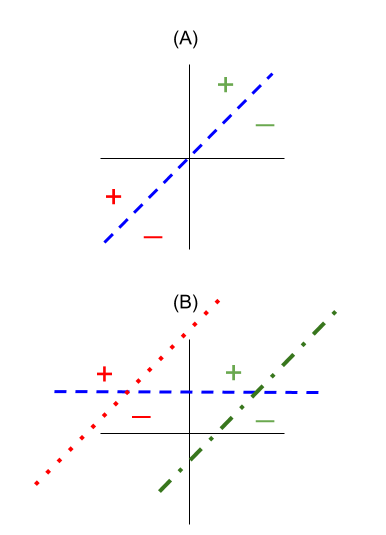
\includegraphics[width=60mm, height=9cm]{graphics/LDA/NegativeExample.png}
\caption{Example of incorrect monitoring by applying LDA locally. The
initial state of the data is presented in (A) and the state at a later point
is shown in (B). In (B) every node (green and red dashed lines) calculates the same angle
for the separator as it was in (A). But it can be
seen that the global separator's (blue solid line) angle has changed
significantly.}
\label{NegativeExample}
\end{figure}


\par To overcome this difficulty, we impose constraints on local data at the nodes, rather than on the function of the global aggregate. Given a function of the average of all local data and the threshold, we compute a ``good'' convex subsets, called \textit{safe zones}, for each node.

\par As we show below, convexity plays a key role in the correctness of this scheme. As long as local data stay inside the safe zones, we guarantee that the function of the global average ---  the euclidean distance between the true global model to the one that was computed in the last synchronization (hereafter, model drift) --- does not cross a threshold.
Nodes communicate only when local data leaves the
safe zone, which we call a safe zone \textit{violation} (hereafter,
violation). Once that happens, violations can be resolved,
for example by synchronization.
In other words, we want to impose conditions on the local
data at each node so that as long as they hold, $||w-w_0||<R_0$, i.e., the global model is valid.

\subsection{Notation}
\noindent
We recall that $P$ and $Q$ are the classes in the binary classification problem.
 $(p,q)$ and $(p^i,q^i)$  are the global and local means of classes $P$ and $Q$.
\\$S$ and $S^i$  are the global and local normalized scatter matrices of the feature space:
\begin{equation*}
S^i := \frac{1}{W}\sum_{j=1}^{W}x^i_j(x^i_j)^T
\end{equation*}
\begin{equation*}
S := \frac{1}{Wk}
\sum_{i=1}^k\sum_{j=1}^Wx^i_j(x^i_j)^T=\frac{1}{k}\sum_{i=1}^kS^i.
\end{equation*}
\\Similarly, $u$ and $u^i$ are the distance between the means of the classes, i.e., $u:=p - q$ and $u^i:=p^i - q^i$.
\\ $B$ is the global covariance matrix, which is the sum of the covariance matrices of the two classes, i.e., $B:=B_p+Bq$.
It can be shown that $B=S - pp^T - qq^T$.
%\\B^i:=S^i - p^i(p^i)^T - q^i(q^i)^T$
\\Let $w$ be our current true model. Then, following Eq.~\ref{eq:w}, we can express:
%\\$w(S,\mu_p,\mu_q) := (S - \mu_p\mu_p^T - \mu_q\mu_q^T)^{-1}(\mu_p - \mu_q)$
\begin{equation}
w:=(S - pp^T - qq^T)^{-1}(p-q)=B^{-1}u.
\end{equation}
%In the following the subscript $0$ will denote the state at the time
%of last synchronization.
Let $w_0$ be the existing model, previously computed from $(S_0, p_0, q_0)$
or from $(B_0,u_0)$ at the time of synchronization.
Then,
\begin{equation}
w_0:=(S_0 - p_0p_0^T - q_0q_0^T)^{-1}(p_0-q_0)=B_0^{-1}u_0.
\end{equation}

If $S_0^i$, $p_0^i$ and $q_0^i$ are the local normalized scatter and averages
of the samples in a node at the time of last synchronization, we define the \textit{local drifts} to be:
\begin{alignat*}{1}
& \Delta_s^i:= S^i - S_0^i
\\ & \delta_p^i:= p^i - p_0^i
\\ & \delta_q^i:= q^i - q_0^i.
\end{alignat*}
We define $\Delta_s, \delta_p$, and $\delta_q$ --- the \textit{global drift} vectors of $S, p$, and $q$ --- to be:
\begin{alignat*}{1}
& \Delta_s:= S - S_0 \\
& \delta_p:= p - p_0 \\
& \delta_q := q - q_0.
\end{alignat*}

\begin{remark} \label{average}
It is easy to see that every global drift vector is the average of the local drift vectors:
\begin{alignat*}{1}
& \Delta_s = \frac{1}{k} \sum \Delta_s^i, \\
& \delta_p = \frac{1}{k} \sum \delta_p^i, \\
& \delta_q = \frac{1}{k} \sum \delta_q^i.
\end{alignat*}

\end{remark}

\subsection{Convex Safe Zones}
Each node monitors its own drift vector: as long as current values
at local nodes $(S^i,p^i,q^i)$ are sufficiently similar to their values
at synchronization time $(S^i_0,p^i_0,q^i_0)$, $w_0$ is guaranteed to be close to $w$.
Formally, we define a convex set $\mathcal{C}$ such that:
\begin{equation} \label{convex}
(\Delta_s, \delta_p, \delta_q) \in \mathcal{C} \Rightarrow \parallel w-w_0
\parallel \ < R_0.
\end{equation}
\begin{lemma} \label{averages}
Let $\mathcal{C}$ be a convex set that satisfies Eq. \ref{convex}.
If $(\Delta_s^i, \delta_p^i, \delta_q^i) \in \mathcal{C}$ for all i, then
\begin{equation*}
||w-w_0|| < R_0.
\end{equation*}
\end{lemma}
\begin{proof}
We express $S, p$ and $q$ as their values at synchronization with the addition of the average of the local drift vectors:
\begin{equation}
\begin{split}
\\(S,p,q) & = \frac{1}{k} \sum_i (S^i,p^i,q^j) \\
 & = (S_0,p_0,q_0) + \frac{1}{k} \sum_i (\Delta_s^i,\delta^i_p,\delta_q^i). \\
\end{split}
\end{equation}
From $\mathcal{C}$'s convexity and using Remark \ref{average} we get:
\begin{equation}
\begin{split}
\forall i (\Delta_s^i,\delta^i_p,\delta_q^i) \in \mathcal{C} & \Rightarrow
\frac{1}{k} \sum_i (\Delta_s^i,\delta^i_p,\delta_q^i) \in \mathcal{C} \\
& \Rightarrow (\Delta_s,\delta_p,\delta_q) \in \mathcal{C}.
\end{split}
\end{equation}
Finally, from the definition of $\mathcal{C}$ we obtain:
\begin{equation}
(\Delta_s,\delta_p,\delta_q) \in \mathcal{C} \Rightarrow \parallel w-w_0
\parallel \ < R_0,
\end{equation}
\end{proof}

\subsection{Convex Bound for Local Condition}
We denote the change in the global covariance matrix
\begin{alignat*}{2}
\Delta & := && B-B_0 \\
& = && (S_0+\Delta_S - (p_0+\delta_p)(p_0+\delta_p)^T \\
& && - (q_0+\delta_q)(q_0+\delta_q)^T) \\
& && - (S_0 - p_0p_0^T - q_0q_0^T) \\
& = && - \delta_p\delta_p^T - \delta_q\delta_q^T \\
& && + \Delta_S - p_0\delta_p^T \\
& && - \delta_pp_0^T - q_0\delta_q^T - \delta_qq_0^T.
\end{alignat*}
We break $\Delta$ into its quadratic part,
\begin{equation*}
M:= - \delta_p\delta_p^T - \delta_q\delta_q^T
\end{equation*}
\begin{equation*}
M^i:= - \delta_p^i(\delta_p^i)^T - \delta_q^i(\delta_q^i)^T
\end{equation*}
and its linear part,
\begin{equation*}
L:= \Delta_S - p_0\delta_p^T - \delta_pp_0^T - q_0\delta_q^T - \delta_qq_0^T
\end{equation*}
\begin{equation*}
\\ L^i := \Delta_S^i - p_0^i(\delta_p^i)^T - \delta_p^i(p_0^i)^T -
q_0^i(\delta_q^i)^T - \delta_q^i(q_0^i)^T,
\end{equation*}
and hence
\begin{equation*}
\Delta= L+ M, 
\end{equation*}
\begin{equation*}
\Delta^i:= L^i+ M^i.
\end{equation*}
We denote the change of the distance between the means as
\begin{equation*}
\delta:= u-u_0 = \delta_p - \delta_q, 
\end{equation*}
\begin{equation*}
\delta^i:=\delta_p^i - \delta_q^i.
\end{equation*}
Now we can define a convex bound for our problem:
\begin{lemma} \label{convexBound}
Let $\mathcal{G}$ be the set of triplets $(\Delta_s^i, \delta_p^i, \delta_q^i)$
 that satisfies the bound:
 \begin{equation} \label{eq:convexBound}
||B_0^{-1}\delta^i|| + \left(||w_0||+R_0)(\Big \| B_0^{-1}L^i \Big \| + \Big \| B_0^{-1}M^i \Big \| \right) \leq  R_0
\end{equation}
where $\Big \| A \Big \|$ is the operator norm of the matrix $A$, and $||v||$ is the euclidean norm of the vector $v$.
\\If $\Big \| B_0^{-1}\Delta^i \Big \| < 1$, then $\mathcal{G}\subseteq \mathcal{C}$ and $\mathcal{G}$ is convex.
\end{lemma}
\subsection{Proof of the Convex Bound Lemma}
\label{sec:appendix1}
We must find a convex subset $\mathcal{C}$ satisfying the condition of Eq. \ref{convex}. Let
us start by recalling the definition of the operator norm of a matrix:
\begin{definition}
Let $A$ be a matrix. Its operator norm or
spectral norm (hereafter just norm), is defined as:
\begin{equation}
\Big \| A \Big \| = \sup_{x \neq 0}\frac{||Ax||}{||x||}.
\end{equation}
\end{definition}
The following result is very useful in the forthcoming analysis:
\begin{lemma} \label{lemma:newman}
If $A$ is square and $\Big \| A \Big \| < 1$, then
\begin{equation*}
\Big \| (I+A)^{-1} \Big \| < \frac{1}{1- \Big \|A \Big \|}.
\end{equation*}
\end{lemma}
The proof for this lemma can be found in \cite{gabel2015monitoring}.

We recall that $\mathcal{C}$ is the convex subset that satisfies
inequality \ref{convex}, and $\mathcal{G}$ is the set of triplets
$(\Delta_s^i, \delta_p^i, \delta_q^i)$
which satisfy the inequality \ref{eq:convexBound}.

\begin{lemma} \label{eq:GinC}
$\mathcal{G} \subseteq \mathcal{C}$

\end{lemma}

\begin{proof}
We can write the sphere inclusion condition \ref{eq:critiria} in terms of $B_0, \Delta, u_0$ and $\delta$, by using the triangle inequality:
\begin{equation} \label{in}
\begin{split}
||w-w_0|| & = \ ||(B_0+\Delta)^{-1}(u_0+\delta) - B_0^{-1}u_0|| \\
& < ||(B_0+\Delta)^{-1}\delta|| \\
& \ \ + ||((B_0+\Delta)^{-1} - B_0^{-1})u_0||.
\end{split}
\end{equation}

We split the right side of the last inequality into two parts:
\begin{equation}  \label{e1e2}
\begin{split}
& E_1:= ||(B_0+\Delta)^{-1}\delta|| \\
& E_2:= ||((B_0+\Delta)^{-1} - B_0^{-1})u_0||.
\end{split}
\end{equation}
Under the assumption  $||B_0^{-1}\Delta||\ \leq \ 1$,
it follows from lemma \ref{lemma:newman}:
\begin{equation} \label{e1e2In}
\begin{split}
& E_1 \leq \frac{||B_0^{-1}\delta||}{1-\Big \|B_0^{-1}\Delta\Big \|} \\
& E_2 \leq  \frac{|| B_0^{-1}\Delta w_0||}{1-\Big \|B_0^{-1}\Delta\Big \|}.
\end{split}
\end{equation}
From standard properties of the norm we get:
\begin{equation} \label{CS}
||B_0^{-1}\Delta w_0||  \leq  \Big \|B_0^{-1}\Delta \Big \| ||w_0||.
\end{equation}
Substituting Eq. \ref{e1e2}, \ref{e1e2In} and \ref{CS} in Eq. \ref{in}, we
get:
\begin{equation}
\begin{split}
|| w-w_0 \parallel & \leq \ E_1+E_2 \\
& \leq \frac{||B_0^{-1}\delta|| + \Big \|B_0^{-1}\Delta\Big \|||w_0||}{1 -\Big \|B_0^{-1}\Delta \Big \|} \\
& \leq R_0.
\end{split}
\end{equation}
After rearranging the terms, we have
\begin{equation} \label{lostDenom}
||B_0^{-1}\delta|| + \Big \|B_0^{-1}\Delta \Big \| ||w_0||
\leq R_0(1 -\Big \|B_0^{-1}\Delta\Big \|).
\end{equation}
From the triangle inequality we can rewrite:
\begin{equation} \label{linQuad}
\Big \|B_0^{-1}\Delta\Big \| \leq \Big \|B_0^{-1}L\Big \|+\Big \|B_0^{-1}M\Big \|.
\end{equation}
And finally, combining inequalities \ref{lostDenom} and \ref{linQuad},
we get the following bound:
\begin{alignat*}{2} \label{convexBound}
&||B_0^{-1}\delta|| &+ (||w_0||+R_0)(\Big \|B_0^{-1}L\Big \|+\Big \|B_0^{-1}M\Big \|)  \leq R_0. \\
&
\end{alignat*}
\end{proof}

\begin{lemma} \label{eq:GisConvex}
$||B_0^{-1}\delta|| + (||w_0||+R_0)(\Big \|B_0^{-1}L\Big \|+\Big \|B_0^{-1}M\Big \|$ is convex in $(\Delta_s,\delta_p, \delta_q).$
%$||B_0^{-1}\delta||$ is convex in $\delta$.
\end{lemma}
\begin{proof}
Multiplication by $B_0^{-1}$ is a linear operation, and norm is a convex
operation. Therefore $||B_0^{-1}\delta||$ is convex in $\delta$.
%\end{proof}

We recall that:
\begin{equation*}
L:= \Delta_S - p_0\delta_p^T - \delta_pp_0^T - q_0\delta_q^T - \delta_qq_0^T.
\end{equation*}
%\begin{lemma} \label{L}
%$||B_0^{-1}L||$ is convex in $\Delta_s, \delta_p$
%and $\delta_q$.
%\end{lemma}
%\begin{proof}
$L$ is linear in $(\Delta_s, \delta_p)$ and therefore $\Big \|B_0^{-1}L\Big \|$ is convex in these variables.

%\end{proof}

We recall that:
\begin{equation*}
M:= - \delta_p\delta_p^T - \delta_q\delta_q^T.
\end{equation*}

%\begin{lemma} \label{M}
It is left to prove that $\Big \|B_0^{-1}M\Big \|$ is convex in $(\delta_p, \delta_q)$.
%\end{lemma}
%\begin{proof}
\\From the definition of the operator norm, we can rewrite:
\begin{alignat*} {2}
\Big \|M \Big \| & = && ||B_0^{-1}(\max_{||u||=1}{\{u^T \delta_p\delta_p^T u\}} +
\max_{||u||=1}{\{u^T \delta_q\delta_q^T u\}})||\\
& = && ||B_0^{-1}(\max_{||u||=1}{\{||u^T \delta_p||^2\}} +
\max_{||u||=1}{\{||u^T \delta_q||^2\}})||.
\end{alignat*}
\\We observe that the maximum over any number (infinite in this case) of convex functions
 is also a convex
function, and since multiplication by a matrix and the norm
operation preserve convexity, this concludes the proof.
\end{proof}

\begin{corollary}
The proofs of Lemmas \ref{eq:GinC} and Lemma \ref{eq:GisConvex} complete the proof of Lemma \ref{eq:convexBound}. From Lemma \ref{eq:convexBound} and from Lemma \ref{averages} we conclude that

\begin{equation}
\begin{split}
(||B_0^{-1}\delta|| + (||w_0||+R_0)(\Big \|B_0^{-1}L\Big \|+\Big \|B_0^{-1}M\Big \|) \\
 \leq R_0) \Rightarrow (||w-w_0|| \leq R_0).
\end{split}
\end{equation}
which validates the convex bound.
\end{corollary}
%
%


\section{Distributed LDA Monitoring Algorithm}
In the following, we present two frameworks for LDA model monitoring that use
the bound in Eq. \ref{eq:convexBound}. 
In both frameworks, 
we define a \textit{coordinator}, whose role is to monitor the violation alerts from the nodes and aggregate the data from all the nodes when it happens. The coordinator recomputes the model after data aggregation and sends the new covariance matrix and the norm of the new model to the nodes.
In both frameworks every node runs the same
update algorithm as detailed in Alg. \ref{NodeUpdate}.
The frameworks differ in their synchronization policy. 
The first, Distributed LDA Monitoring (DLDA), will synchronize in a round
in which at least one node has reported a violation (condition \ref{eq:convexBound} in the node is not satisfied) as detailed in Alg.~\ref{DLDA}).
The second, Probabilistic Distributed LDA Monitoring (PDLDA), will synchronize in a round in which the number of nodes with a violation is above a certain
threshold.
The derivation of this threshold is presented Section \ref{sec:PDLDA}.

\begin{algorithm}
\caption{Node Update: $i$ is the index of the node, $(x,y)$ is a new sample.}
\label{NodeUpdate}
\begin{algorithmic}[1]
\Procedure{Update}{}
\If {$y$ is class P}
\State $p^i = p^i + x - x_{old}^i(p)$
\State $S^i = S^i +xx^T - x_{old}^i(p)*(x_{old}^i(p))^T$
\Else
\State $q^i = q^i + x -x_{old}^i(q)$
\State $S^i = S^i +xx^T - x_{old}^i(q)*(x_{old}^i(q))^T$
\EndIf
\State $(\Delta_s^i,\delta^i_p,\delta_q^i) = (S^i-S^i_0,p^i-p^i_0,q^i-q^i_0)$
%\If{The bound in \ref{eq:convexBound} is not satisfied}

\If { \begin{varwidth}[t]{\linewidth}
$||B_0^{-1}\delta^i||+ (||w_0||+R_0)(||B_0^{-1}L^i||+||B_0^{-1}M^i||) $ \par
\hskip\algorithmicindent $>R_0$}
\end{varwidth}
\State Report violation to coordinator
\State Receive new global $B_0^{-1}$, $||w_0||$
\State $(S_0^i,p_0^i,q_0^i) = (S^i,p^i,q^i)$
\EndIf

\EndProcedure
\end{algorithmic}
\end{algorithm}

\begin{algorithm}
\caption{Coordinator synchronization algorithm.}\label{DLDA}
\begin{algorithmic}[1]
\Procedure{Sync}{}
\If {One of the nodes has reported for violation}
\State Ask from the nodes for their data
\State Receive from every node $i$ the triplet $(S^i,p^i,q^i)$
\State Compute updated $||w_0||$ and $B_0^{-1}$ and distribute.
\EndIf
\EndProcedure
\end{algorithmic}
\end{algorithm}

\subsection{Probabilistic Distributed LDA Monitoring}\label{sec:PDLDA}

DLDA triggers synchronization when a single node reports a violation.
Our empirical evaluation with a large number of nodes showed that such a strict
policy causes synchronization even when the global model is still valid. Loosely speaking, it is because the condition in Equation \ref{eq:convexBound} is stricter than the original condition from Equation \ref{eq:critiria}. Formally, it appears that in most of the datasets, $\mathcal{G}$ (the  convex subset of $\mathcal{C}$) is a \textit{proper} subset of $\mathcal{C}$, and usually much smaller. To resolve this problem, we suggest to change the synchronization policy of the system and synchronizing when a certain portion of nodes report a violation.
This portion is learned empirically on the training set of the system and is notated as VT.
%
%
\subsection{Analysis of the probabilistic version, PDLDA}
%

\section{Evaluation}
%
We evaluated the performance of the proposed monitoring algorithms, DLDA and PDLDA, on synthetic and real data. For each dataset we simulated a distributed data stream by partitioning the data between the nodes and streaming it one sample in a round. 

\subsection{Synthetic Data Experiments}
We use synthetic data, in which all model assumptions hold, to
exemplify the communication efficiency of our method (Section \ref{sec:com_eff})
and its ability to decide that the model isn't valid {\emph before} the
misclassifications (Section \ref{sec:earlydetection}). We then (Section \ref{sec:paramanal}) analyze the communication efficiency of our method as a function of the algorithm parameters.
%
%
\subsubsection{Communication Efficiency}\label{sec:com_eff}
We compare DLDA to the $T$-periodic algorithm, denoted
PER($T$), a sampling algorithm that sends updates
every $T$ rounds.
Our main performance metric is communication, measured in \textit{normalized messages} (the average number of messages sent per round by each node). 
PER can achieve arbitrarily low communication at the cost of larger model drift. However,
periodic synchronization can miss the point of change in the data; 
hence PER cannot guarantee to maintain the model drift under a fixed threshold, in contrast to DLDA.  Further,
DLDA has additional intrinsic advantages over PER: 
\begin{enumerate}
\item DLDA can be instantly calibrated to fit a given drift threshold, while for PER the 
interval between synchronizations can only be determined empirically. 
\item The rate that the data evolves might change. 
While DLDA adapts to the new changing rate, PER suffers from its fixed period
that has to be suboptimal to the new one.
\item For a sudden change in the data, DLDA adapts immediately --- the algorithm's
\textit{latency} is 0 --- while for PER the latency might be up to the period length.
\end{enumerate}

In this experiment we used a simple data generation process. There are 10 nodes, each of which contains two data classes: $P$, a Gaussian centered
at the origin and with unit covariance matrix; and $Q$, a Gaussian also
with unit covariance matrix, but whose mean changes every 1,500 rounds, starting at $(1,0)$, and then changing to $(0,-1), (-1,0), (0,1)$ (see 
Fig. \ref{DataShiftInEarlyDetection}.

\begin{figure}[ht]
\label{DataShiftInEarlyDetection}
	\centering
	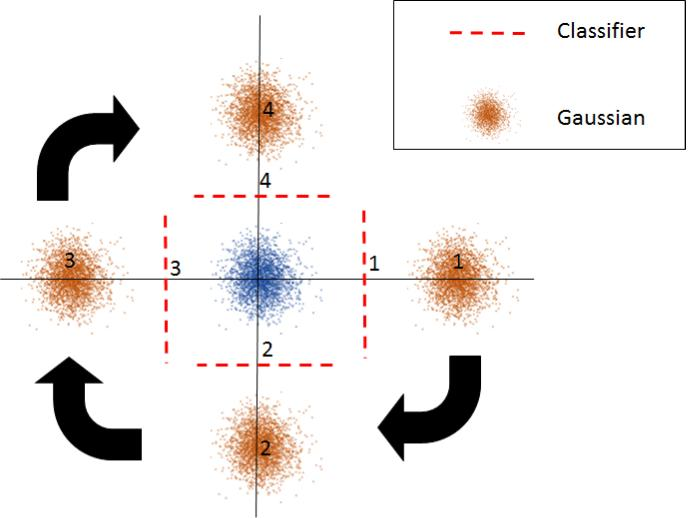
\includegraphics[width=9cm, height=7cm]{graphics/LDA/DataShiftInEarlyDetection.jpg}
	\caption{Illustration of the generation process of the synthetic data.
	The class $P$ (denoted in blue) is fixed, while $Q$ changes three
	times, every 1,500 rounds (the changes are depicted by the dark arrows).
	\ref{PERvsDLDAoverTime}.}
	\label{DataShiftInEarlyDetection}
\end{figure}

Figure \ref{PERvsDLDAoverTime} shows the behavior of the DLDA monitoring
algorithm over the synthetic dataset, with three points in time at which the data abruptly changes. 
DLDA achieves a communication overhead of 0.01 messages per node per round, with the model error guaranteed to always be below the given threshold.
Conversely, the equivalent PER(100) algorithm doesn't maintain the
model error below the threshold (red dashed line).
Figure \ref{PERvsDLDAoverTime} shows that the periodic algorithm does not always 
synchronize when the model drift exceeds a given threshold. 
Moreover, it triggers redundant synchronizations when there is no change in the data.
\begin{figure*}[ht]
	\centering
	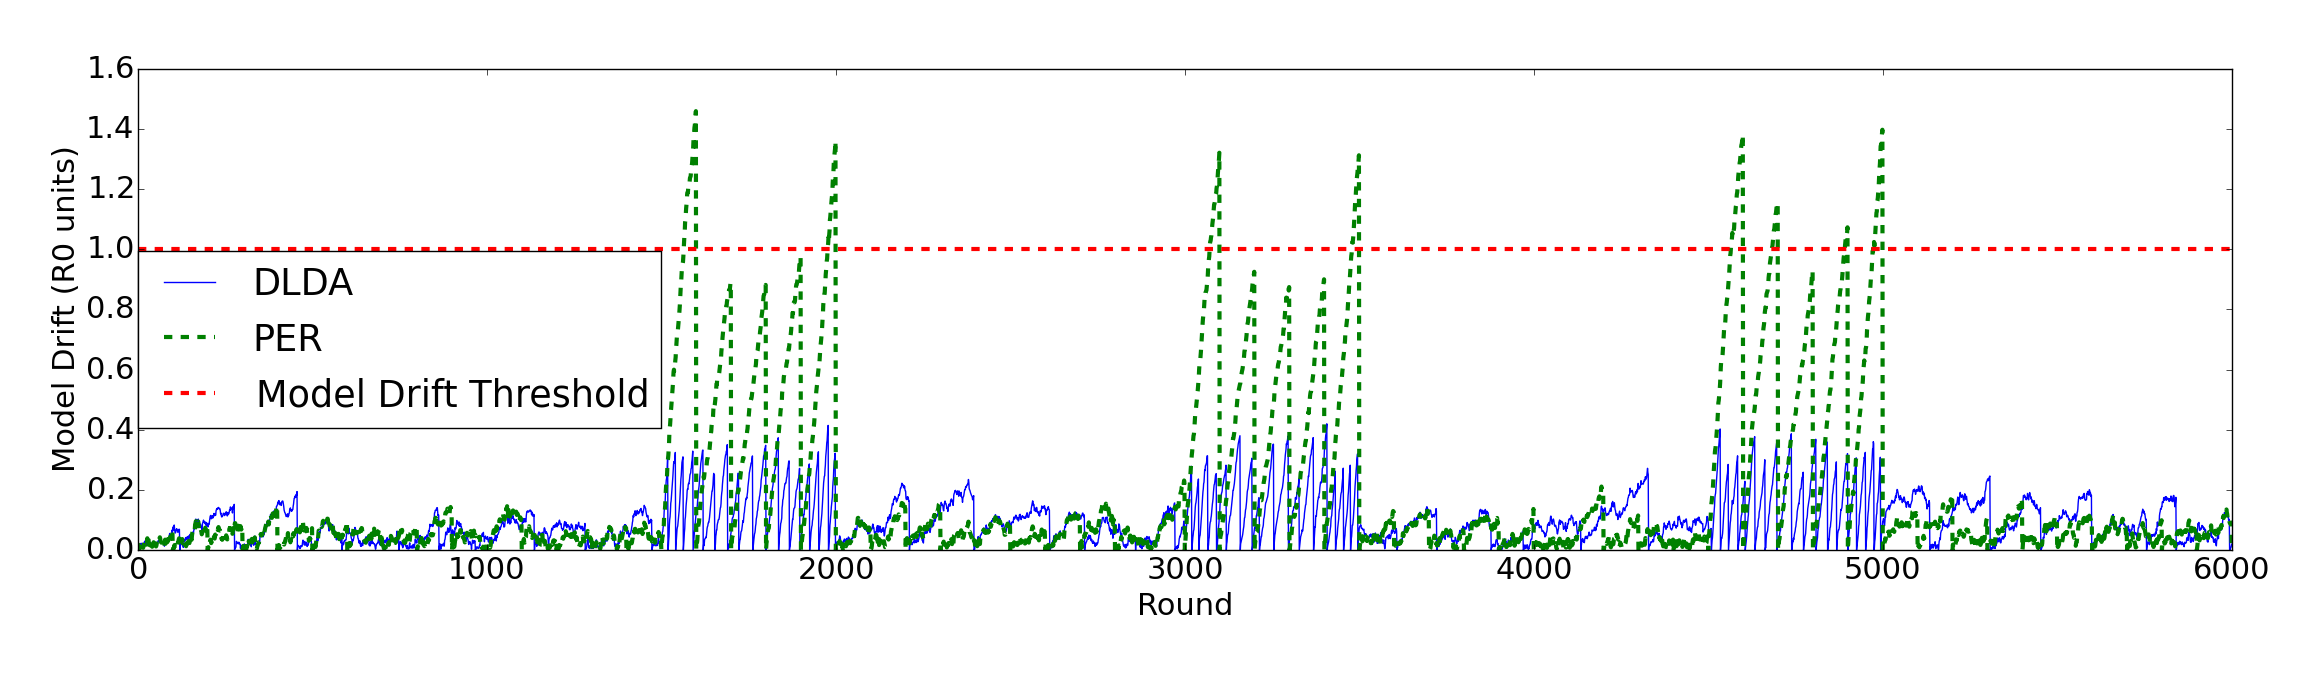
\includegraphics[width=\textwidth, height=7cm]{graphics/LDA/PERvsDLDAoverTime.png}
	\caption{DLDA error (blue) vs. PER(100) error (red), for the synthetic
	data described above. Horizontal axis represents rounds, vertical
	axis represents the norm of the difference between the real (global) model and the current model held at the nodes. Window size is 1,000.
	The maximum allowed error (which DLDA guarantees will never be
	surpassed) is $T = 0.997$ (which corresponds to a difference of
	0.077 radians, or 4.4 degrees, in the classifier's direction). Both
	algorithms transmit the same overall number of bytes, but at different
	rounds; while PER sends alerts periodically, DLDA alerts only when the classifier may have changed. For this reason, PER yields a larger
	error when the two classes (and the classifier) change.
}
	\label{PERvsDLDAoverTime}
\end{figure*}
%
%
\subsubsection{Early Drift Detection}\label{sec:earlydetection}
%
%
To further expound on the advantage of the proposed DLDA algorithm, we consider a toy example (Fig. \ref{EarlyDetection}), 
in which 2D data arrives from two classes ($P$'s samples are shown as plus signs and $Q$'s samples as minus signs). The means of the classes change 
according to the depicted grey arrows, from time $t_1$ to $t_L$. The dark
line at an angle of $-45^{\circ}$ represents the optimal projection
direction at time $t_1$. As the classes change, this initial projection
direction remains "correct", in the sense that it still separates the
two classes; alas, at time $t_L$, the two classes have switched their
positions relative to the projection's direction, and the classifier
fails. Hence, a monitoring algorithm which only checks for misclassification
at the nodes will fail to detect the drift in the classes until it is too
late -- i.e., that the classifier fails -- while DLDA will alert earlier, 
when the real (global) classifier will have changed by more than the
provided threshold (in this case 0.52 radians, or $30^{\circ}$); this point is marked by an arrow in Fig. \ref{EarlyDetection}.
%
\begin{figure}[ht]
	\centering
	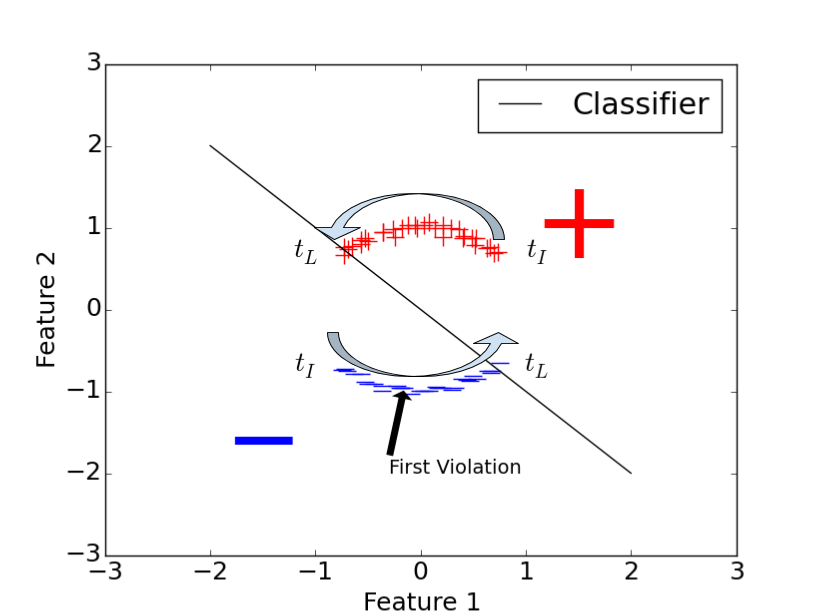
\includegraphics[width=90mm, height=7cm]{graphics/LDA/EarlyDetection.png}
	\caption{A toy example demonstrating early detection of a change in the data.}
	\label{EarlyDetection}
\end{figure}
%
%
\subsubsection{Parameter Analysis}\label{sec:paramanal}
Next, we analyze the parameters of the DLDA algorithm.

\noindent\textbf{Model Drift Threshold:} Model Drift Threshold is given by the user. Above it the model drift is too big. It can be quantified in two ways: as the maximal angle between $w$ and $w_0$, or as the euclidean distance between them. 
Figure \ref{PERvsDLDAoverError} shows the communication requirements of the DLDA algorithm as a function of the model drift threshold, and the minimal communication required to match DLDA using PER.	
It can been seen that for both fixed and dynamic data, DLDA outperforms PER for
any given model drift threshold.
 \begin{figure*}
	\centering
	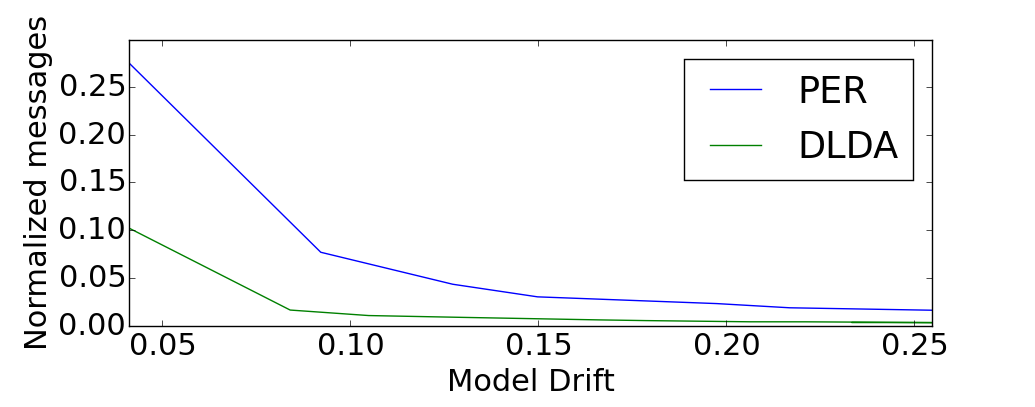
\includegraphics[width=110mm, height=5cm]{graphics/LDA/onlyDrift.png}
	\caption{Communication as the function of model drift for DLDA and PER. The
	periodic algorithm is tuned to achieve the same max model drift as DLDA
	for each model drift threshold.}
	\label{PERvsDLDAoverError}
\end{figure*}

	
\noindent\textbf{Node Scalability:}
Node Scalability is how DLDA performs with different number of nodes.
Figure \ref{Nodes} shows the communication volume as a function of the number of nodes $k$.
We observe that communication increases slowly, reaching 0.25\% on the fixed
data and 0.6\% on the dynamic data distributed across 25 nodes.

\begin{figure}[]
\centering
    \centering
  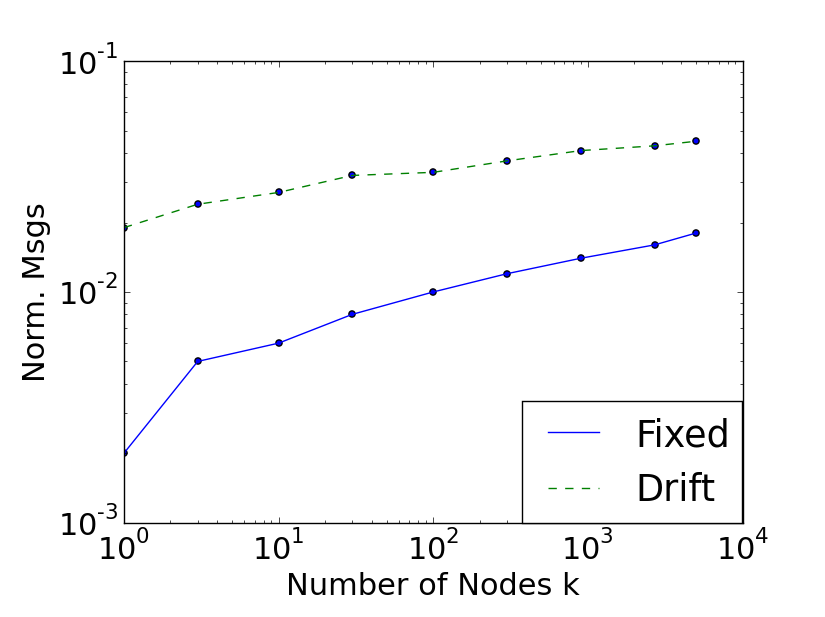
\includegraphics[width=90mm]{graphics/LDA/Nodes.png}
  \caption{Communication as a function of the number of nodes for fixed (blue)
  and changing (green dashed line) datasets}\label{Nodes}
  \end{figure}
 \begin{figure}[]
\centering
  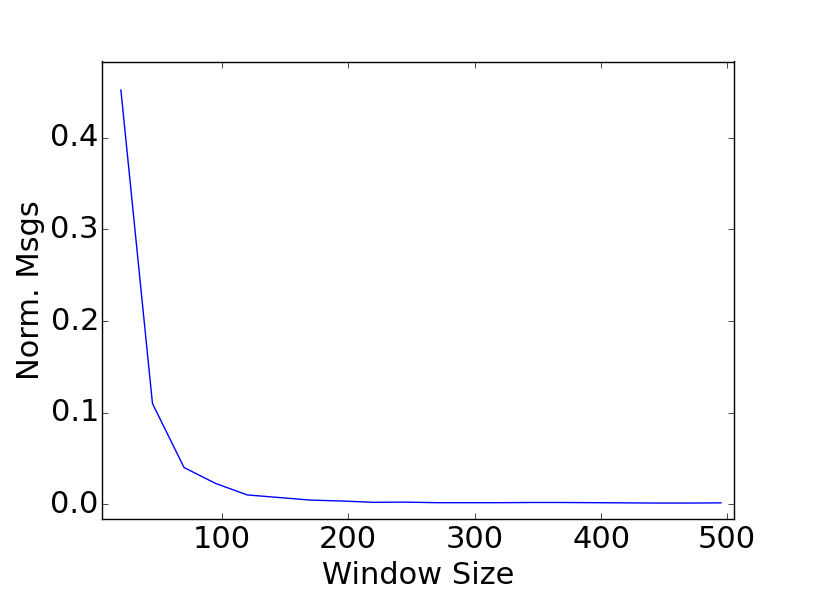
\includegraphics[width=90mm]{graphics/LDA/WindowSize.png}
  \caption{Communication as function of window size }\label{WindowSize}
  \end{figure}
  
  \begin{figure}[]
\centering
  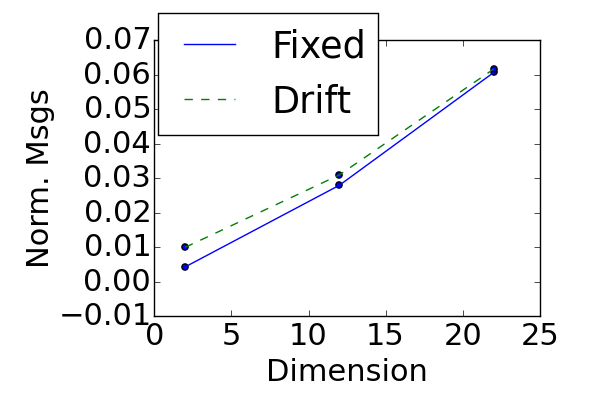
\includegraphics[width=90mm]{graphics/LDA/Dimension.png}
  \caption{Communication as a function of input dimension for fixed (blue) and
  changing (green  dashed line) datasets}\label{Dimension}
\end{figure}

\noindent\textbf{Window Size:}
Figure \ref{WindowSize} shows how communication decreases as a result
of enlarging the window size $W$.  One can increase the window size to compensate for other factors in the system that increase the communication. One of those is
noise (which is quantified in our context by the standard deviation of the
data generating distribution).

%\subsubsection{Noise}
%Figure \ref{Noise} shows normalized messages obtained for different
%noise magnitudes. The experiment shows that the drift grows with the noise, causing more %synchronizations (more communication). This result is not surprising, and the solution is to increase the window size.

Another parameter directly related to the window size is the dimension of the data. The number of samples required for accurate estimation of the covariance matrix grows with the dimension. In our settings, the number of training samples is linked to the window size. When window size is fixed, communication grows linearly with the dimension (see Figure \ref{Dimension}).



\begin{figure}
	\centering
	\includegraphics[width=3.5in,height=2in]{graphics/LDA/DriftDetected.png}
	%\includegraphics[width=\textwidth]{Usenet/DriftDetected.png}
	\caption{Comparison between maximal (over nodes) DLDA model drift (blue)
	and the true global model drift (green dashed line) for $k=2$, $W=450$.
	It can be seen that DLDA responds to the change in the data that occurs
	after 600 rounds (red dotted vertical line) and causes a synchronization in round 698 (blue dashed vertical line).}
	\label{usenet}
	\end{figure}
\subsection{Real Data Experiments}
In this section we test the algorithm on three real data sets. The first
(USENET) is too small to test the probabilistic approach; thus we use this set only for the DLDA test.
The second (Power Consumption Monitoring) is a medium size dataset (it
is distributed over 36 nodes) and we test both DLDA and PDLDA on it.
The third (Gas Sensor Time Series Monitoring) is a big set(it is distributed over
100 nodes). The DLDA synchronization policy is too strict for a large number of nodes; hence we use this set only for the PDLDA test.

\subsubsection{Message Preference Monitoring --- Usenet}
The USENET dataset (~\ref{usenet}) is a text dataset that simulates a stream of messages 
from three newsgroups (medicine, space, baseball); 
the messages are presented sequentially to a user, who then labels them as interesting or junk, 
according to personal interest. 
Attribute values are binary, indicating the presence or absence of the 128 informative words. 
The change in the data occurs from a change in the user's preference (from space to baseball). 
Figure \ref{usenet} shows the results of the DLDA algorithm with $W=450$ . The first 450 rounds over the data correspond to
the initialization phase and are omitted. During the next 50 rounds the DLDA model drift 
(the value is calculated using the left side of the inequality in Eq. \ref{eq:convexBound}) 
increases due to noise in the data; there is no change in the user's
preferences.
From round 500 to 600 the DLDA model drift is stable, and again is due only to the noise. In round 600 there is a concept
drift.
From this point both the DLDA model drift and the true model drift increase until the synchronization in round 698.
\subsubsection{Power Consumption Monitoring}
The Power Consumption dataset contains the hourly power supply of an
Italian electric company as recorded from two sources: power supplied
by the main grid and power transformed from other grids.
This stream contains three-year power supply records
from 1995 to 1998, and our learning task is to predict which hour (1 out of 24 hours) 
the current power supply belongs to. 
Thchange in the dataft in this stream is mainly caused by such factors as season, weather, time of day,
and the differences between working days and weekend.
We demonstrate the algorithms on the following binary classification problem:
given a power supply measurement, decide whether it corresponds to night or day.
This dataset is an example of gradual change in the data (seasons do not
change abruptly).
Figure \ref{PowerSupplyFigures} depicts the results of the DLDA
and PDLDA algorithms. For a small number of nodes, $k=4$, and for large
window size, $W=5000$, DLDA requires only 0.003 normalized messages.
For a more distributed system, $k=36$, and a smaller window
size, $W=600$, DLDA requires 0.09 normalized messages. For PDLDA with
$k=36$ and $W=600$ and a violation threshold (VT) of 50\%, PDLDA
requires 0.02 normalized messages, much better than DLDA in the same setting.

\begin{figure*}
    \centering
    \begin{subfigure}[b]{0.8\textwidth}
        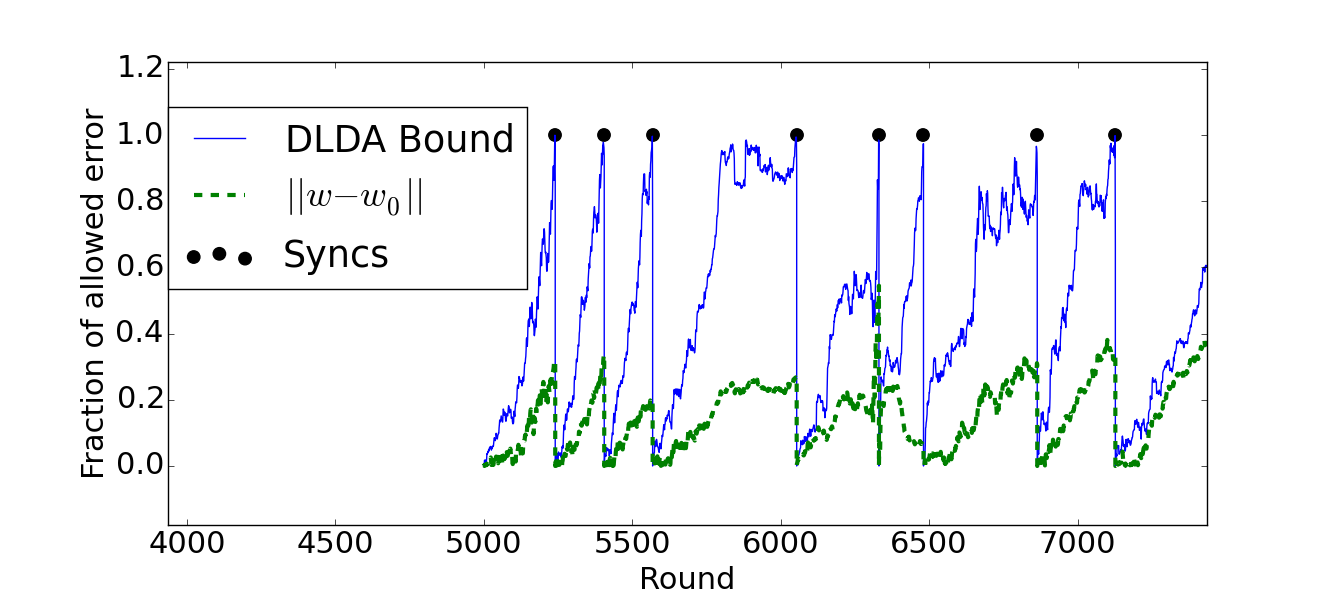
\includegraphics[width=\textwidth]{graphics/LDA/4nodes.png}
        \caption{DLDA behavior on Power Consumption data with: k=4, W=5000, VT=0}
    \end{subfigure}

    \begin{subfigure}[b]{0.8\textwidth}
        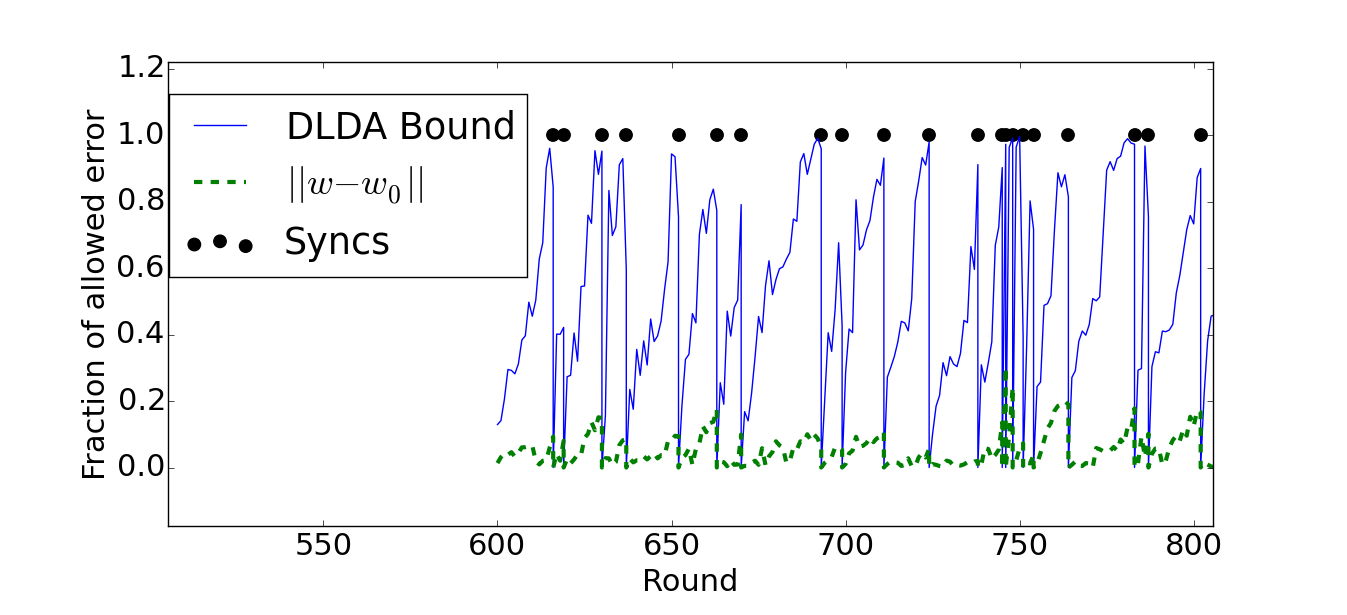
\includegraphics[width=\textwidth]{graphics/LDA/36nodes.png}
        \caption{DLDA behavior on Power Consumption data with: k=36 Nodes, W=600, VT=0}
    \end{subfigure}

    \begin{subfigure}[b]{0.8\textwidth}
        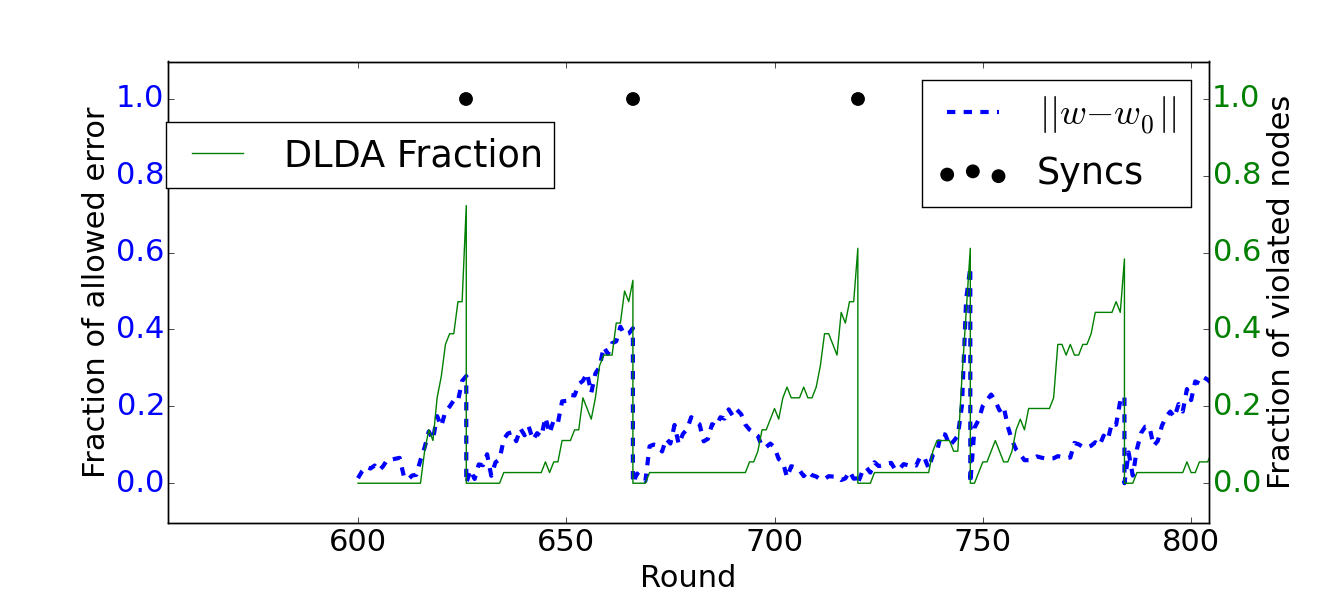
\includegraphics[width=\textwidth]{graphics/LDA/36nodesProb.png}
        \caption{PDLDA behavior on Power Consumption data with: k=36 Nodes, W=600, VT=18}
    \end{subfigure}
    \caption{The top and the center figures show the DLDA algorithm on the Power Supply data set for a small (top) and large (center) number of nodes. The blue line represents the value of the local bound expression, corresponding to the node with the maximum value. The green dashed line shows the model drift (normalized by the threshold); the model is computed after the data was aggregated from all nodes. The bottom plot shows the results of the PDLDA on the same dataset. The blue line in the bottom plot represents the fraction of violated nodes.}\label{PowerSupplyFigures}
\end{figure*}

\subsubsection{Gas Sensor Time Series Monitoring}
\begin{figure*}
\centering
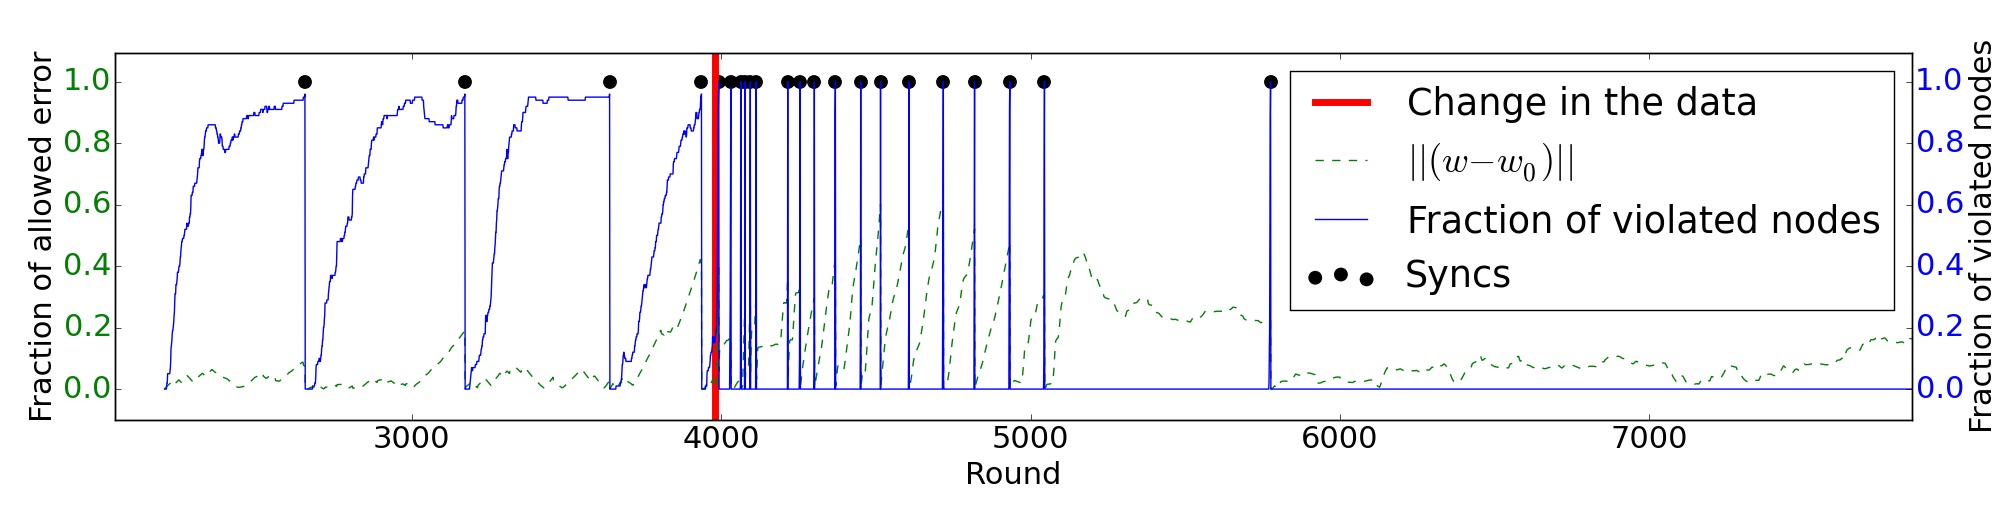
\includegraphics[width=\textwidth]{graphics/LDA/overTime100k.png}
\caption{Demonstration of PDLDA on the Gas Sensor dataset.
A comparison between the true model drift (green) to the fraction of the nodes that
are violated in the current round (blue).
The experiment is configured for k=100 nodes, and the violation threshold is
VT=80.}
\label{BigGasOverTime}
\end{figure*}
Data in this experiment consists of measurements collected
by an array of 16 chemical sensors in a lab, recording at a sampling
rate of 100Hz for 24 hours, resulting in 8378504 data points for each sensor.
During the first 12 hours the task is to detect the presence of carbon monoxide
(CO) in a mixture of chemicals, and from the 13th hour the task is to detect the presence of methane, 
which corresponds to an abrupt change in the data.
Figure \ref{BigGasOverTime} demonstrates the results of PDLDA algorithm.
First, we can observe that the fraction of violated nodes (shown in blue) correlates with the true model drift (shown in green). Second, we can see two patterns of behavior, which are separated by an abrupt switch in the data  (marked by the vertical red line). Before the switch,  the synchronization occurs every 150 rounds, and after the switch, it goes down to every 50 rounds. There is a transition period of about 1000 rounds that follows the point of the data switch. In this interval, the sliding window mixes the old (before switch) data and the new (after the switch) data, but once the window aggregates enough data, the algorithms stabilizes and reduces the communication requirements.   This experiment shows that the PDLDA algorithm detects the abrupt change in the data and adapts to the new conditions after a short period of time.







\thesisbibfiles{bib}
\thesisbibstyle{alpha}





% end of file template.tex

